\documentclass[a4paper]{article}
\usepackage[utf8]{inputenc}
\usepackage[spanish, es-tabla, es-noshorthands]{babel}
\usepackage[table,xcdraw]{xcolor}
\usepackage[a4paper, footnotesep = 1cm, width=20cm, top=2.5cm, height=25cm, textwidth=18cm, textheight=25cm]{geometry}
%\geometry{showframe}

\usepackage{tikz}
\usepackage{amsmath}
\usepackage{amsfonts}
\usepackage{amssymb}
\usepackage{float}
\usepackage{graphicx}
\usepackage{caption}
\usepackage{subcaption}
\usepackage{multicol}
\usepackage{multirow}
\setlength{\doublerulesep}{\arrayrulewidth}
\usepackage{booktabs}

\usepackage{hyperref}
\hypersetup{
    colorlinks=true,
    linkcolor=blue,
    filecolor=magenta,      
    urlcolor=blue,
    citecolor=blue,    
}

\newcommand{\quotes}[1]{``#1''}
\usepackage{array}
\newcolumntype{C}[1]{>{\centering\let\newline\\\arraybackslash\hspace{0pt}}m{#1}}
\usepackage[american]{circuitikz}
\usetikzlibrary{calc}
\usepackage{fancyhdr}
\usepackage{units} 

\graphicspath{{../Ejercicio-1/}{../Ejercicio-2/}}

\pagestyle{fancy}
\fancyhf{}
\lhead{22.67 - Señales Aleatorias}
\rhead{Lambertucci, Londero B., Moriconi, Musich, Tolaba}
\rfoot{Página \thepage}

\begin{document}

Utilizando el método de simulación de Montecarlo, se obtiene que, dado $X$, un cariable aleatoria uniforme entre 0 y 1, se puede obtener una distribución exponencial $Y$ mediante la función densidad de probailidad
\begin{equation}
	y(x) = \frac{1}{\lambda} ln\left( \frac{1}{1 - x} \right) \ \ \ \ 0 \leq x \leq 1
\end{equation}

Valiendose de las funciones hist, mean y std de Matlab, y asignando arbitrariamente un valor a lambda, en este caso $\lambda = 2$, luego de una simulación se obtienen los siguientes resultados:
\begin{figure}[H]
	\centering
	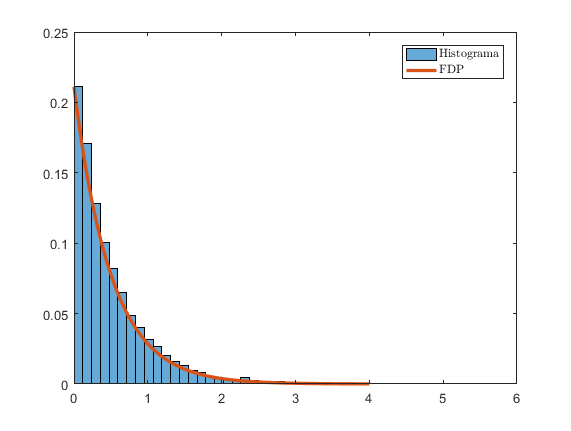
\includegraphics[width=0.7\linewidth]{./ImagenesEjercicio1/Simu-1.png}
	\caption{Iteración del método de Montecarlo.}
	\label{fig:primerit}
\end{figure}

\begin{equation}
\begin{aligned}
		\mu_{Y} = & \ 0.5048 \\
		{\sigma_{Y}}^{2} = & \ 0.2617
\end{aligned}
\end{equation}

Es así que se observa en la Figura (\ref{fig:primerit}) la curva de la fdp teórica sobre el histograma obtenido, confirmando así que se obtuvo realmente una variable aleatoria con la distribución deseada. Además, se desea constatar que los valores de $\mu_{Y}$ y ${\sigma_{Y}}^{2}$, son correctos. Por ser $Y$ una V.A. exponencial, se sabe que $\mu_{Y} = \frac{1}{\lambda} = 0.5$ y ${\sigma_{Y}}^{2} = \frac{1}{\lambda^2} = 0.25$, para el caso presentado. Si bien los resultados obtenidos no son exactamente iguales, son proximos, siendo dicho error aceptable.  

\end{document}